Tässä luvussa käsitellään ensin työhön keskeisesti kuuluvan verkkoteorian perusteita ja käydään huolellisesti läpi niistä tässä työssä käytettävät osat.
Työssä sovelletaan erityisesti verkkoteorian painotettua verkkoa sekä verkkoteoriassa esiintyvän lyhimmän polun ongelmaan kehitettyä Dijkstran algoritmia.
Verkkoteoria itsessään on osa diskeettiä matematiikkaa.

Verkkoteorian jälkeen tässä luvussa esitetään vaiheittain työn tuloksena kehitetty priorisointimenetelmä.
Priorisointia varten esitetään harkintaa käyttäen valitut priorisointiin vaikuttavat muuttujat, niitä käyttävät painofunktiot, verkon rakentaminen ja karsiminen sekä verkon ja testitapauksien yhteys.
Lisäksi käydään läpi miten menetelmää käyttäen tuotetun painotetun verkon sisältämää informaatiota voidaan hyödyntää prioriteeteiltaan tärkeimmän polun löytämiseen \ref{ch:10_dijkstran_algoritmin_hyodyntaminen}.

\section{Matemaattisten verkkojen tarkoitus} \label{ch:09_matemaattisten_verkkojen_tarkoitus}

  Matemaattisten verkkojen tarkoituksena on mallintaan parittaisia riippuvuuksia verkkomaisessa objektijoukossa.
  Verkkoteoriassa peruskäsitteitä ovat itse \emph{verkko} eli \emph{graafi}, joka muodostuu \emph{solmuista} ja niiden välisiä riippuvuuksia esittävistä \emph{kaarista} tai \emph{nuolista}.
  Verkkoteorialla on lukuisia käytännön sovellutuksia. Verkkoteoriaa sovelletaan muun muassa tietokonetieteissä, kielitieteissä, fysiikan ja kemian sovellutuksissa, sosiaalisissa tieteissä ja biologiassa.
  Alun perin verkkoteoria katsotaan syntyneen 1700-luvulla esiintyneestä niin sanotusta Königsbergin siltaongelmasta, johon Leonhard Euler esitti todistuksensa.

  Matemaattisten verkkojen käyttöön päädyttiin tässä työssä siksi, että niiden avulla on hyväksymistestauksen kohteena oleva käyttöliittymä mahdollistaa mallintaa verkoksi.
  Käyttöliittymän verkkomuotoiseen esitykseen voidaan vielä lisätä painot, jotka tässä tapauksessa kuvaavat prioriteetteja, mahdollistaen testikokoelmien priorisoinnin.

\section{Perusmerkinnät ja käsitteet} \label{ch:09_perusmerkinnat_ja_kasitteet}

  Verkkoteoriassa käytetään muun muassa seuraavia perusmerkintöjä ja käsitteitä:

  \begin{itemize}
    \item \(V := \{v_1, v_2, v_3\}\) Solmujoukko joka sisältää \emph{solmut} \(v_1\), \(v_2\) ja \(v_3\).
    \item \(E := \{e_1, e_2, e_3\}\) Kaarijoukko joka sisältää \emph{kaaret} \(e_1\), \(e_2\) ja \(e_3\).
    \item \(\phi(e_1) := \langle v_1, v_2 \rangle\) Kaariparin \(v_1\) ja \(v_2\) yhdistävän \emph{kaaren} \(e_1\) kuvaaja.
    \item \(d_G(x)\) Solmun asteluku, eli solmuun liittyvien \emph{kaarten} määrä.
    \item \(G_2 \subset G_1\) Aliverkko, eli \emph{verkko} \(G_2\) joka koostuu osasta \emph{verkon} \(G_1\) \emph{solmuja} ja \emph{kaaria}.
    \item \(v_1 \neq v_2, v_1 \rightarrow v_2\) Verkon yhtenäisyys, eli jokaiselle solmuparille \(v_1 \neq v_2\) on olemassa niitä yhdistävä \emph{kaari}.
    \item \(P = \{v_0, v_1, ..., v_n\}, v_0 \rightarrow v_n\) Polku, eli \emph{suunnattu solmujono} jota pitkin voidaan kulkea \emph{solmusta} \(v_0\) \emph{solmuun} \(v_n\).
    \item \(P = \{v_0, v_1, ..., v_n| e \in E_P, e \notin \{E_P \setminus \{e\} \}\}\) Sykli, eli \emph{polku}, jonka aloitus \(v_0\) ja lopetussolmu \(v_n\) on sama, mutta polun jokaista kaarta \(e\) kuljetaan vain kerran.
    \item \(d_G(v_1) = 0\) Eristetty solmu, eli \emph{solmu} jonka \emph{asteluku} on nolla.
    \item \(v_1 \rightarrow v_2, d_G(v_1) = 1 \lor d_G(v_2) = 1\) Silta, eli \emph{kaari} johon yhdistyvän \emph{solmun asteluku} on yksi ja jonka poistaminen epäyhteinäistää \emph{verkon}.
    \item \(v_x \rightarrow v_x\) Silmukka, eli \emph{kaari} jonka \emph{aloitussolmut} ja \emph{lopetussolmu} ovat sama \emph{solmu}.
    \item \(\alpha := V(G), E(G) \rightarrow \mathbb{N}\) Painofunktion yleinen kuvaus verkossa \(G\), solmuille \(V\) ja kaarille \(E\).
  \end{itemize}

\section{Priorisointiin vaikuttavat muuttujat} \label{ch:10_priorisointiin_vaikuttavat_muuttujat}

  Näkymä- ja siirtymäperustaiseen priorisointiin vaikuttavat monet eri asiat, joista osa kasvattaa prioriteettia ja osa laskee sitä.
  Prioriteettia kasvattava muuttuja on esimerkiksi liiketoiminnallinen arvo ja laskeva muuttuja on esimerkiksi projektin muutosherkkyys.
  Muuttujat ovat kuitenkin hyvin kontekstiriippuvaisia, joten yleispätevää ja kaikkiin tilanteisiin soveltuvaa listaa muuttujista on hankala antaa.
  Kontekstiriippuvaisuuden takia muuttujiin ja myöhemmin esitettäviin painofunktioihin on varattu paikka omille lisämuuttujille.

  Tässä diplomityössä esiteltävää priorisointimenetelmää varten jokainen priorisointiin vaikuttava muuttuja arvioidaan asteikolla 1-10, paria poikkeusta lukuun ottamatta.
  Numeerisella asteikolla on tarkoitus antaa korkea numero, jos muuttuja on prioriteetiltaan tärkeä kyseisen näkymän, eli verkon solmun kohdalla.
  Jos jokin muuttuja ei ole kelpoinen siinä kontekstissa, jossa menetelmää yritetään hyödyntää, tulee muuttujan arvo asettaa nollaksi, jolloin se sivuutetaan painofunktiossa \ref{ch:10_painofunktiot_priorisointiin}.

  Poikkeukselliset muuttujat ovat käyttötapauksien määrä ja siirtymien määrä, joissa numeerisen asteikon sijaan käytetään kyseisten muuttujien määrää suhteessa koko verkkoon.
  Esimerkiksi siirtymien määrää ilmaiseva suhde määritetään laskemalla solmun asteluku \(d_G(v)\), eli solmuun liittyneiden kaarien määrä, jaettuna kaikilla verkossa olevien kaarien määrällä.
  Lisäksi siirtymien määrän suhde vielä kerrotaan luvulla 10, jotta se saadaan skaalautumaan muiden muuttujien kanssa samalle tasolle.

  \begin{table}[H]
    \caption{Priorisointiin vaikuttavat muuttujat}
    \label{tab:priorisointiin_vaikuttavat_muuttujat}
    \centering
    \begin{tabular}{lllll} \hline
    \(m\) & \textbf{Muuttuja} & \textbf{Etumerkki} & \textbf{Asteikko} &  \\ \hline
    \textbf{1} & Liiketoiminnallinen arvo & \(+\) & 1 - 10 &  \\
    \textbf{2} & Liiketoiminnallinen visio & \(+\) & 1 - 10 &  \\
    \textbf{3} & Negatiivinen käyttäjäpalaute & \(+\) & 1 - 5 &  \\
    \textbf{4} & Käyttötapauksien määrä & \(+\) & 10 \(\cdot\) suhde &  \\
    \textbf{5} & Siirtymien määrä & \(+\) & 10 \(\cdot\) suhde &  \\
    \textbf{6} & Positiivinen käyttäjäpalaute & \(-\) & 1 - 5 &  \\
    \textbf{7} & Muutosherkkyys & \(-\) & 1 - 10 &  \\
    \textbf{8} & Toteuttamisen kompleksisuus & \(-\) & 1 - 5 &  \\
    \textbf{9} & Toteutuksen virheherkkyys & \(-\) & 1 - 5 &  \\
    \textbf{10} & Omat lisämuuttujat & \(\pm\) & 1 - 10 & \\ \hline
    \end{tabular}
  \end{table}

\section{Painofunktiot priorisointiin} \label{ch:10_painofunktiot_priorisointiin}

  Painofunktioiden määrittäminen on tärkeä osa painotetun verkon avulla priorisointia, sillä niiden avulla määritetään verkon solmujen ja kaarien prioriteetit.
  Tavanomaisesti numeerinen prioriteetti usein mielletään olevan korkea, jos priorisoitu muuttuja on tärkeä.
  Painotettujen verkkojen tapauksessa on kuitenkin järkevää vaihtaa numeerisen prioriteetin suuntaa, jotta painotettuun verkoon sovellettavat lyhimmän polun algoritmit toimisivat etsien prioriteetiltaan tärkeitä polkuja. Ennen prioriteetin suunnanvaihtoa, voidaan kokonaisprioriteetti \(p\) yksittäiselle solmulle \(v\), eli näkymälle määrittää seuraavasti.

  \[p(v) = \sum\limits_{i=1}^{5} m_i - \sum\limits_{j=6}^{9} m_j \pm m_{10}\]

  Prioriteetin suunnan vaihtamiseksi suuresta pieneen, säilyttäen kuitenkin prioriteetin sisältämän informaation, voi hoitaa käänteislukujen avulla.
  Ennen käänteisluvuksi muuttamista, prioriteettiin vaikuttavien muuttujien yhteenlaskettu summa voi olla ongelmallisesti negatiivinen tai nolla.
  Negatiiviset arvot eivät ole painotetun verkon kannalta erityisen järkeviä, sillä tässä diplomityössä hyödynnettävää Dijkstran algoritmia ei voida käyttää negatiivisien painojen kanssa.
  Dijkstran algoritmin toiminta nollan tapauksessa voi myös kuulostaa epäilyttävältä, kuten esimerkiksi tilanne, jossa painotetun verkon kaikki painot olisivat nollia.
  Dijkstran algoritmin tapauksessa tällainen verkko on kuitenkin sallittu, koska silloin lyhimmän polun ratkaisu on verkon kaikki solmut.
  Lyhimmän polun ongelman erityisvaatimusten lisäksi käänteislukua varten nolla on huono arvo siinä mielessä, että sille ei ole olemassa lainkaan käänteislukua.
  Tämä johtuu siitä, että jos nollalle yrittäisi etsiä käänteislukua, tulisi eteen nollalla jakaminen jota ei voi tehdä.
  Nämä molemmat ongelmatapaukset voidaan kuitenkin painofunktiossa ratkaista siten, että käänteisfunktiota ei etsitä, vaan korvataan painofunktion tulos yhdellä.

  Painofunktio yksittäiselle solmulle \(v\), eli näkymälle saadaan solmun kokonaisprioriteetin \(p(v)\) käänteislukuna.

  \[\alpha(v) = \begin{cases}
    p^{-1}(v) & p(v) > 0 \\
    1 & p(v) \leq 0
  \end{cases}\]

  Painofunktio yksittäiselle solmut \(v_x\) ja \(v_y\) yhdistävälle kaarelle \(e_{xy}\), eli siirtymälle saadan myös käänteislukuna.
  Kaaren painofunktiota varten pitää kuitenkin huomioida, että sen kokonaisprioriteetti on kaaren solmujen kokonaisprioriteetin summa \(p(v_x) + p(v_y)\).
  Kaaren kokonaisprioriteetti \(p(v_1) + p(v_2)\) pitää laskea ennen käänteisluvuksi muuttamista.

  \[\beta(e_{xy}) = \begin{cases}
    (p(v_x) + p(v_y))^{-1} & p(v_x) + p(v_y) > 0 \\
    1 & p(v_x) + p(v_y) \leq 0
  \end{cases}\]

\section{Verkon rakentaminen} \label{ch:10_verkon_rakentaminen}

  Tässä diplomityössä on aiemmin moneen otteeseen kerrottu näkymä ja siirtymäperusteisesta testiautomaation toteuttamisesta ja priorisoinnista.
  Painotetun verkon rakentamista varten tulee tarvittavat näkymät ja niiden väliset siirtymät muodostavat testauskohteen käyttöliittymästä.
  Web-sovelluksen käyttöliittymän näkymiä ovat muun muassa sivut, sivujen sisältämät säiliö-elementit ja dialogit.
  Siirtymät ovat usein sivujen välisiä linkkejä tai vaihtoehtoisesti jotakin sellaista toiminnallisuutta, joka muuttaa nykyisen näkymän tai osan siitä toiseksi näkymäksi.

  Seuraavassa taulukossa on esitetty kuvitteellisen web-sovelluksen mukainen näkymien ja siirtymien mukaan laadittu esimerkki \ref{tab:esimerkki_verkon_priorisointi_muuttujat}.
  Taulukossa esitetään näkymät kirjautumisnäkymästä ohjenäkymään ja jokaisen näkymän siirtymät eli yhteydet toisiin näkymiin.
  Näkymät ja siirtymät luovat matemaattisen verkon laatimisen perusedellytykset, eli datan jonka avulla myöhemmin esitettävä painomatriisi voidaan laatia.
  Taulukossa on lisäksi esitetty jokainen näkymään liittyvä priorisointiin vaikuttava muuttuja.
  Priorisointiin vaikuttavien muuttujien arvot on laadittu subjektiivisesti kuvitteellisen esimerkin muodossa.
  Priorisointiin vaikuttavien muuttujien yhteenlaskettu prioriteetti yksittäiselle näkymälle on laskettu taulukkoon valmiiksi käyttäen aiemmin esitettyä prioriteettifunktiota \(p(n)\), jossa \(n\) tarkoittaa sitä näkymää jolle prioriteetti lasketaan.

  \begin{table}[H]
    \caption{Esimerkkiverkon näkymät, siirtymät ja priorisointimuuttujat}
    \label{tab:esimerkki_verkon_priorisointi_muuttujat}
    \centering
    \begin{tabular}{lllllllllllll} \hline
    \(n\) & \textbf{Näkymä} & \textbf{Siirtymät} & \(m_1\) & \(m_2\) & \(m_3\) & \(m_4\) & \(m_5\) & \(m_6\) & \(m_7\) & \(m_8\) & \(m_9\) & \(p(n)\) \\ \hline
    \textbf{A} & Kirjautuminen & B & 10 & 10 & 0 & 2 & 1 & 0 & 5 & 5 & 5 & 8 \\
    \textbf{B} & Pelivalikko & A, C, D, G & 8 & 10 & 1 & 2 & 4 & 4 & 5 & 5 & 5 & 6 \\
    \textbf{C} & Asetukset & A, B & 4 & 6 & 5 & 2 & 2 & 2 & 5 & 5 & 5 & 2 \\
    \textbf{D} & Peli & B, E, G & 10 & 10 & 4 & 2 & 3 & 4 & 4 & 5 & 5 & 11 \\
    \textbf{E} & Tulokset & B, D, F & 6 & 8 & 0 & 2 & 3 & 5 & 5 & 4 & 5 & 2 \\
    \textbf{F} & Onnittelu & B, E & 1 & 8 & 0 & 0 & 2 & 2 & 5 & 2 & 5 & -3 \\
    \textbf{G} & Ohje & B, D & 1 & 10 & 2 & 0 & 2 & 0 & 8 & 0 & 0 & 7 \\ \hline
    \end{tabular}
  \end{table}

  Painotetun verkon rakentamisen syötteeksi täytyy käyttöliittymän näkymät ja siirtymät sekä niiden painoarvot esittää painomatriisin muodossa.
  Painoarvot saadaan aiemmin esitetyn painofunktion \(\beta\) avulla \ref{ch:10_painofunktiot_priorisointiin}.
  Painoarvo lasketaan \(\beta\) funktion avulla jokaiselle kahta näkymää yhdistävälle siirtymälle, eli painotetun verkon solmujen väliselle kaarelle.
  Painofunktio \(\beta\) käyttää kaaren molempien päätepisteiden \(v_A\) ja \(v_B\) yhteenlaskettua prioriteettia, josta käänteisluku otetaan.
  Näin saadaan laskettua kaarelle sellainen painoarvo, joka tarkoittaa painotetussa verkossa siirtymän näkymiin sidottua prioriteettia.

  \[\beta(e_{AB}) = (p(v_A) + p(v_B))^{-1} = (8 + 6)^{-1} = \frac{1}{14} \approx 0.071\]

  Painomatriisi, esimerkin mukaiselle datalle \ref{tab:esimerkki_verkon_priorisointi_muuttujat} ja siitä lasketuille painoarvoille on esitetty seuraavassa matriisissa \(M_G\).
  Painomatriisissa tulee väistämättä esiin tilanne, jossa pitää määrittää painoarvo kaarelle jonka aloitussolmu ja lopetussolmu ovat sama solmu itsessään.
  Tällaisissa tapauksissa, tilanteesta riippuen painomatriiseihin usein merkitään \(0\), \(\infty\) tai \(-\).
  Tässä diplomityössä esitettävän menetelmän painomatriiseissa solmuun itseensä johtuvan kaaren, eli silmukan painoksi merkitään aina \(-\), koska käyttöliittymän näkymästä siirtymät itseensä ei menetelmässä käsitellä aitoina siirtyminä.
  Tämän lisäksi luonnollisesti jokainen sellainen solmupari, jolla ei ole niitä yhdistävää kaarta merkitään painomatriisiin käyttäen \(-\) merkintää.
  Sellaisien siirtymien toiminnallisuuden testaaminen on tarkoitus kattaa näkymän mukaisen testikokelman testitapauksissa ja ne tulee priorisoiduiksi näkymä ja siirtymäperusteisesti.
  Painotetun verkon kaaret voivat verkkoteorian mukaan olla suunnattuja tai suuntaamattomia.
  Tässä esimerkkitapauksessa jokainen siirtymä näkymien välillä on suuntaamaton, eli toisin sanoen käyttöliittymässä kaksisuuntainen ja se priorisoidaan sen mukaisesti.
  Painomatriisissa suuntaamattomien kaarien johdosta voidaan huomata, että painomatriisin diagonaalin erottamat puoliskot ovat toistensa peilikuvia.

  \[
    M_G \approx
    \bordermatrix{
      G   & v_A   & v_B   & v_C   & v_D   & v_E   & v_F   & v_G   \cr
      v_A & -     & 0.071 & 0.100 & -     & -     & -     & -     \cr
      v_B & 0.071 & -     & 0.125 & 0.059 & 0.125 & 0.333 & 1.000 \cr
      v_C & 0.100 & 0.125 & -     & -     & -     & -     & -     \cr
      v_D & -     & 0.059 & -     & -     & 0.077 & -     & 0.250 \cr
      v_E & -     & 0.125 & -     & 0.077 & -     & 1.000 & -     \cr
      v_F & -     & 0.333 & -     & -     & 1.000 & -     & -     \cr
      v_G & -     & 1.000 & -     & 0.250 & -     & -     & -     \cr
    }
  \]

  Painomatriisin avulla voidaan siis rakentaa matemaattinen painotettu verkko, joka kuvaa näkymiä ja siirtymiä sekä niiden prioriteetteja.
  Painotetun verkon kuvaamiseen piirretään jokainen erilaista käyttöliittymän näkymää vastaava ja esimerkkidatan \ref{tab:esimerkki_verkon_priorisointi_muuttujat} mukainen solmu ja niiden välisiä siirtymiä kuvaavat yhteydet eli kaaret.
  Kaarien yhteyteen lisätään kuvaajassa kaaren prioriteettia kuvaava painoarvo.
  Seuraavassa on esitetty painomatriisin dataa vastaava painotetun verkon kuvaaja \ref{fig:painotettu-verkko-ennen} sellaisena, kuin se on ennen siihen tehtäviä prioriteettileikkauksia.
  Priorisoimista varten tehtävien leikkauksien tekeminen esitetään myöhemmin omassa kappaleessaan \ref{ch:10_verkon_karsiminen}.

  \begin{figure}[H]
    \centering
    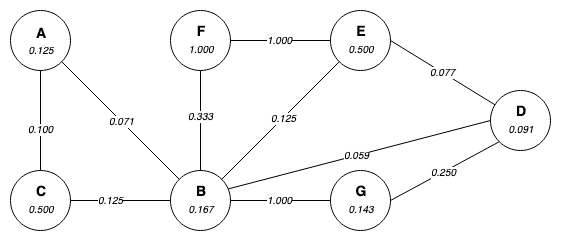
\includegraphics[width=0.6\textwidth]{assets/painotettu-verkko-ennen.png}
    \caption{Esimerkki painotetusta verkosta ennen leikkauksia}
    \label{fig:painotettu-verkko-ennen}
  \end{figure}

  Perinteisesti painotetuissa verkoissa ei esitetä yksittäisiä solmupainoja vaan painotetun verkon painoilla tarkoitetaan solmujen välisien kaarien painoarvoja.
  Tässä diplomityössä kehitettyä menetelmää käytettäessä edellä esitettyyn painotettuun verkkoon \ref{fig:painotettu-verkko-ennen} on kuitenkin lisätty painomatriisin sisältämän informaation lisäksi painofunktion \(\alpha(v)\) avulla lasketut yksittäisten solmujen eli näkymien painoarvot.

  \[\alpha(v_A) = p^{-1}(v_A) = 8^{-1} = \frac{1}{8} = 0.125\]

  Yksittäisten solmujen prioriteettia kuvaavat painoarvot ovat erittäin merkittäviä ja hyödyllisiä, sillä niiden avulla voidaan järjestää itse solmut, eli näkymät prioriteettien mukaiseen järjestykseen.
  Tämän lisäksi solmujen prioriteettien avulla voidaan verkkoon muun muassa soveltaa lyhimmän polun ratkaisemiseen kehitettyjä algoritmeja, kuten myöhemmin Dijkstran algoritmin osalta esitetään omassa kappaleessaan \ref{ch:10_dijkstran_algoritmin_hyodyntaminen}.

\section{Verkon karsiminen} \label{ch:10_verkon_karsiminen}

  Painotetun verkon karsiminen eli leikkaaminen on prioriteeillä painotetun verkon tärkeä ominaisuus.
  Verkkoteorian soveltaminen prioriteettien avulla painotettuun verkkoon on erityisen hyödyllistä, kun verkon kaarissa alhainen paino tarkoittaa suurta prioriteettia.
  Verkon karsimista varten valitaan kattavuus, joka vastaa minimirajaa ja jonka jälkeen karsiminen lopetetaan.
  Kattavuus tarkoittaa myös testikattavuutta testikokoelmien näkökulmasta, sillä painotetussa verkossa jokainen solmu, eli näkymä vastaa näkymän mukaan kategorisoitua testikokoelmaa.

  Verkkoon tehtäviä leikkauksia varten tarvitsee määrittää haluttu kattavuus \(0 \leq c \leq 100\), joka on prosentuaalinen luku siitä kuinka suuri osa verkon solmuista eli näkymistä tai testikokoelmista täytyy verkkoon jäädä karsimisen jälkeenkin. Leikkauksien tekeminen ja toistaminen suoritetaan käyttäen seuraavia toimenpiteitä \(n\)-kertaa, niin kauan kunnes karsittu aliverkko on suurempi kuin kattavuuden mukaan laskettu osuus alkuperäisestä verkosta tai jos iteraatiokerralla ei enää löydy toimenpiteillä poistettavia solmuja.
  \[|V(G_s)| > c \cdot \frac{|V(G)|}{100}, G_s \subset G\]

  Tässä verkon karsimisen esimerkissä kattavuutena käytetään \(c = 80\), joka tarkoittaa esimerkin solmujen määrän \(7\) karsimista \(80 \cdot \frac{7}{100} = 5.6\), eli lukumäärään \(5\) asti.

  \begin{enumerate}
    \item Poistetaan verkosta löytyvä eristetty solmu, eli solmu jonka asteluku on nolla.
    \[d_G(v) = 0\]
    \item Poistetaan verkosta löytyvä sillattu solmu, eli solmu jonka asteluku on yksi ja paino on pienempi kuin solmujen painojen keskiarvo.
    \[d_G(v) = 1  \land \alpha(v) > \frac{1}{|V(G)|} \cdot \sum\limits_{v \in V(G)} \alpha(v)\]
    \item Poistetaan verkosta sellainen alhaisimman prioriteetin solmu, jonka asteluku on pienempi kuin solmujen astelukujen keskiarvo ja paino on pienempi kuin solmujen painojen keskiarvo.
    \[d_G(v) < max\{d_G(x) | x \in V(G)\} \land \alpha(v) > \frac{1}{|V(G)|} \cdot \sum\limits_{v \in V(G)} \alpha(v)\]
  \end{enumerate}

  \begin{figure}[H]
    \centering
    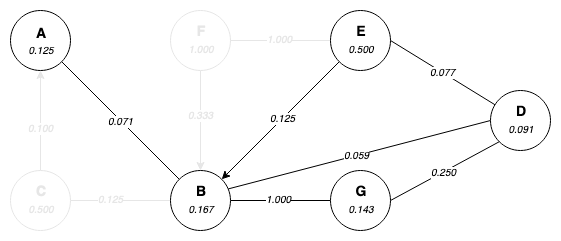
\includegraphics[width=0.6\textwidth]{assets/painotettu-verkko-jalkeen.png}
    \caption{Esimerkki painotetusta verkosta leikkauksien jälkeen}
    \label{fig:painotettu-verkko-jalkeen}
  \end{figure}

\section{Dijkstran algoritmin hyödyntäminen} \label{ch:10_dijkstran_algoritmin_hyodyntaminen}

  Priorisointimenetelmän mukaan karsittuun painotettuun verkkoon on mahdollista soveltaa lyhimmän polun ongelman ratkaisemiseen kehitettyjä algoritmeja, jolloin ne toimivat etsien alhaisimman, eli korkeimman prioriteetin polkuja.
  Lyhimmän polun etsimiseen on tarkoitus valita aina sellaiset aloitus ja lopetuspisteet, joiden välille lyhin polku verkossa halutaan etsiä.
  Lyhimmän polun löytymisen yhtenä perusedellytyksenä on verkon yhtenäisyys, joka tarkoittaa sitä, että verkon kaikkia solmuja tulee yhdistää vähintään yksi kaari ja että verkon jokaisesta solmusta on löydettävissä yhteys mihin tahansa verkon solmuun.
  Lyhimmän polun ongelma johon muun muassa Dijkstran algoritmi antaa ratkaisun on matemaattisessa muodossaan seuraavanlainen.

  \[d_G^\alpha(v_1, v_2) = min\{\alpha(P) | P:v_1 \rightarrow v_2 | v_1, v_2 \in V(G)\}\]

  Prioriteeteiltaan tärkeimmän polun löytämiseksi, valitaan ensin \(min\{\alpha(v_1) | v_1 \in V(G)\}\) ja \(min\{\alpha(v_2) | v_2 \in V(G), v_1 \neq v_2\}\) sekä etsitään sitten Dijkstran algoritmin avulla niiden välinen lyhin polku.
  Dijkstran algoritmin sisäinen toimintaperiaate ei ole tämän diplomityön näkökulmasta oleellista, mutta se on kuitenkin esitetty tarkemmin pseudokoodina liitteessä \ref{ch:13_liite_dijkstran_algoritmi}.
  Dijkstran algoritmi kahdelle painoltaan pienimmälle, eli prioriteetiltaan korkeimmalle antaa tuloksena \(v_1\) ja \(v_2\) solmuja yhdistävän polun, jonka sisältävät solmut eli näkymät ovat prioriteetiltaan tärkeimmät.
  Koska painotetun verkon painofunktiot on laadittu käänteislukuja hyödyntäen, Dijkstran algoritmi löytää painoarvoltaan matalimman, mutta prioriteetiltaan tärkeimmän polun solmujen \(v_1\) ja \(v_2\) välille.
  Näin ollen saadaan helposti ja vaivattomasti tietää sellaiset solmut eli käyttöliittymän näkymät jotka kuuluvat tärkeimpiin ja joista testiautomaation rakentaminen kannattaa aloittaa.

\section{Verkon ja testitapauksien yhteys} \label{ch:10_verkon_ja_testitapauksien_yhteys}

  Ennen testitapauksien suunnittelua tehtävä painotetun verkon avulla tehty priorisointi havainnollistaa käyttöliittymän näkymiä ja niiden välisiä siirtymiä.
  Tällaisesta painotetusta verkosta saadaan priorisoitua näkymät ja siirtymät, mutta lopulliset testitapauksien prioriteetit ovat kuitenkin testitapaukseen kuuluvien näkymien tai siirtymien prioriteetteja.
  Tämä tarkoittaa käytännössä sitä, että kun näkymät ja siirtymät on priorisoitu, on esimerkiksi yhden yksittäisen tarkasteltavana olevan näkymän toiminnoilla sama keskenään prioriteetti.
  Painotetun verkon näkymät ovatkin suoraan yhteydessä testiautomaatiota varten rakennettaviin testikokoelmiin, jotka sisältävät kokoelman testitapauksia kyseiselle näkymälle.
  Toisin sanoen, painotetun verkon näkymiä vastaavat testikokoelmat ovat varsinaisen priorisoinnin kohteena.

  Testitapaukset ja testikokoelmat kappaleessa \ref{ch:07_testitapaus_ja_testikokoelmat} on esitetty niiden välistä eroa ja sitä kuinka testikokoelmat koostuvat yhteen liittyvistä testitapauksista.
  Painotetun verkon avulla tehtävää priorisointia käyttäessä on tarkoitus ajatella testiautomaation testitapauksien kategorisoimista testikokoelmiksi käyttöliittymän näkymiä vastaavalla tavalla.
  Kun käyttöliittymän näkymillä on niitä vastaavat testikokoelmat, toimii tässä diplomityössä kehitetty painotetun verkon avulla toteutattava priorisointi oikein ja siten kuin se on tarkoitettu.
  Jos testiautomaation halutaan lisätä testitapauksia tai testikokoelmia, jotka eivät ole luettavissa painotetusta verkosta, niille ei luonnollisesti ole olemassa prioriteettia ja sellaiset täytyy käsitellä ylimääräisinä, täydentävinä testitapauksina.

  Painotetun verkon kuvaamisen seurauksena, voidaan verkosta nähdä myös paljon hyödyllistä informaatiota, kuten muun muassa siinä esiintyviä sillattuja solmuja sekä syklejä.
  Sillatut solmut ovat sellaisia käyttöliittymän näkymiä, joihin käyttäjä ei kovinkaan usein päädy ja näin ollen jos niitä lopullisessa karsitussa verkossa esiintyy, ne ovat testiautomaatin rakentamisen kannalta usein vain vähän merkitseviä.
  Eristetyt solmut ovat samaan tapaan vain vähän merkitseviä kuin sillatut solmut.
  Syklit puolestaan ovat erittäin merkittävä osa painotetussa verkossa ja testiautomaation rakentamisessa, sillä ne ovat sellaisia käyttöliittymän näkymiä ja niiden välisiä siirtymiä, jotka toistuvat käyttäjälle usein käyttöliittymää käyttäessään.
  Solmujen asteluvut kertovat myös paljon solmujen merkitsevyydestä.
  Sellainen solmu jonka asteluku, eli siihen liittyvien kaarien lukumäärä on korkea, on testiautomaation rakentamisen kannalta yhtälailla erittäin merkittävä osa testiautomaatiota.
